\documentclass{article}

\title{	
	\normalfont\normalsize 
	\rule{\linewidth}{0.5pt}\\ % Thin top horizontal rule
	\vspace{14pt} % Whitespace
	{\LARGE MATH428 Assignment 3 \\ % The assignment title
    \large \textit{} \\}
	\vspace{6pt} % Whitespace
	\rule{\linewidth}{1pt}\\ % Thick bottom horizontal rule
}

\author{Elliott Hughes}
\date{\normalsize\today}
\usepackage{tikz}
\usepackage{tikz-3dplot}
\usetikzlibrary{arrows,automata}
\usetikzlibrary{positioning}
\usetikzlibrary{arrows.meta,positioning}
\usetikzlibrary{calc}
\usetikzlibrary{shapes.geometric}


\usepackage{mdframed}
\usepackage{amsmath}
\usepackage{amssymb}
\usepackage{graphicx}
\graphicspath{ {./Images/} }
\usepackage{commath}
\usepackage{textcomp}
\usepackage{gensymb}
\usepackage{float}
\usepackage{hyperref}
\usepackage[margin=1in]{geometry}
\usepackage{caption}
\usepackage{subcaption}
\usepackage{sectsty}
\usepackage{titlesec}
\usepackage{rotating}
\usepackage{pgfplots}

\begin{document}

\maketitle

\section*{Q1}
\subsection*{(a)}
Consider the map 

\begin{equation*}
    R(x,y,z) = (x,y,-t + (1-t)z)
\end{equation*}

defined on both these spaces. It is hopefully clear that this is a deformation retraction 
from $W$ to $E^2\backslash\{p\}$ (for some $p$ in the interior of $E^2$) and from $W^+$ to $E^2$. However 
$E^2\backslash\{p\} \sim S^1$ and so 

\begin{equation*}
    W \sim E^2\backslash\{p\} \sim S^1 \nsim E^2 \sim W^+
\end{equation*}

Since these spaces are not homotopic, they cannot be homeomorphic.

\subsection*{(b)}
It is relatively straightforward to construct these spaces as CW complexes (see \autoref{fig:Q1_cells}).

\begin{figure}[H]
    \centering
    \begin{subfigure}[b]{0.4\textwidth}
        \centering
    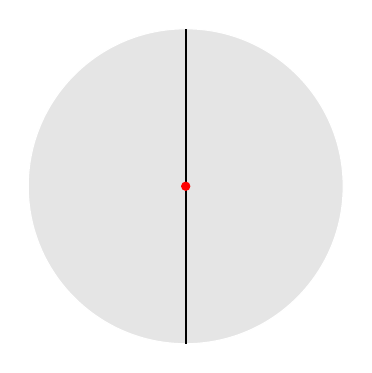
\begin{tikzpicture}

        % Define center points
        \filldraw[fill = black!10, draw = black!0] (0,0) circle(2);
        \draw[thick] (0,0) -- (0,2);
        \draw[thick] (0,0) -- (0,-2);
        \node[fill = red, circle, inner sep = 1.2] (top_orig) at (0,0) {};
    \end{tikzpicture}
    \caption{$\mathring{E}^2$}
    \end{subfigure}
    \begin{subfigure}[b]{0.4\textwidth}
        \centering
    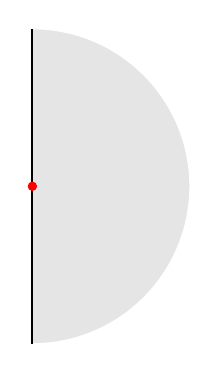
\begin{tikzpicture}

        % Define center points
        \filldraw[fill = black!10, draw = black!0] (0,-2) arc(-90:90:2) -- cycle;
        \draw[thick] (0,0) -- (0,2);
        \draw[thick] (0,0) -- (0,-2);
        \node[fill = red, circle, inner sep = 1.2] (top_orig) at (0,0) {};
    \end{tikzpicture}
    \caption{$\mathring{E}^2_+$}
    \end{subfigure}
      \caption{$\mathring{E}^2$ and $\mathring{E}^2_+$ as cell complexes.}
      \label{fig:Q1_cells}
\end{figure}

It is hopefully now obvious that $\chi(\mathring{E}^2) = 1$ and $\chi(\mathring{E}^2_+) = 0$ 
and so these spaces cannot be homeomorphic.

\section*{Q2}
\subsection*{(a)}
For $f:T \rightarrow K$ and $g:K\rightarrow T$ continuous functions on path connected spaces, if $f \circ g \sim 1_K$ 
then it follows from Lemma 2 that  

\begin{equation*}
    (f\circ g)_* = h^* \circ 1_K = h^*
\end{equation*}

for some isomorphism $h^*$. However, $g_*$ is an isomorphism from $\pi_1(K) = \langle g,k:gk = kg^{-1} \rangle$ to $\pi_1(T) = \mathbb{Z}\times \mathbb{Z}$ 
so we obtain 

\begin{equation*}
    g_*(gk) = g_*(kg^{-1}) \implies g_*(g)g_*(k) = g_*(k)g_*(g^{-1}) = g_*(g^{-1})g_*(k) \implies g^*(g) = g_*(g)^{-1}
\end{equation*}

and thus $g_*(g)$ must have order one or two. Since there is only such element in $\mathbb{Z} \times \mathbb{Z}$ (the 
identity element) it is hopefully obvious that $g_*(\pi_1(K)) = \mathbb{Z}$. Thus $f_*\circ g_*(\pi_1(K))$ is a 
quotient group of $\mathbb{Z}$. Since the quotient groups of $\mathbb{Z}$ are Abelian it follows 
that $f_*\circ g_*(\pi_1(K)) < \pi_1(K)$. Thus $(f \circ g)_*$ is not an isomorphism and so $f \circ g \nsim 1_K$.

\subsection*{(b)}
Since for $f:T \rightarrow K$ and $g:K\rightarrow T$ continuous functions, $f \circ g \nsim 1_K$ 
it follows that these spaces cannot be homotopic and thus cannot be homeomorphic.

\section*{Q3}
\subsection*{(a)}
% Suppose $f:S^1 \times S^1 \rightarrow C \subset S^1 \times S^1$ where $C$ is homeomorphic to the 
% circle $S^1$. Then if $C$ is a deformation retract of $S^1 \times S^1$ it follows that $f$ is 
% homotopic to the identity map $1_T$. Since $S^1 \times S^1$ is path connected it follows that 
% lemma 2 that for $f_*$ the group homomorphism induced by $f$

% \begin{equation*}
%     f_* = h_* \circ 1_T
% \end{equation*}

% for some isomorphism $h_*:\pi_1(S^1 \times S^1) \rightarrow \pi_1(S^1\times S^1)$. 
It is straightforward to construct a retraction from $S^1 \times S^1$ to $C$ homeomorphic to 
$S^1$. Considering $S^1 \times S^1$ expressed in polar coordinates, the map 

\begin{equation*}
    r(\theta,r,\phi) = (\theta,1,\pi/2)
\end{equation*}

is clearly continuous and maps all points in $S^1\times S^1$ to $\{(\theta,1,\pi/2):\theta \in [0,2\pi)\}$.
Since this subspace is also fixed under $r$ this is a retraction.

\paragraph{}
By the second implication of Corollary 3, $C$ homeomorphic to $S^1$ is a deformation 
retraction of $S^1 \times S^1$ if and only if their fundamental groups are isomorphic. However, 
since $\pi_1(S^1) = \mathbb{Z}$ is cyclic and $\pi_1(S^1 \times S^1) = \mathbb{Z} \times \mathbb{Z}$ 
is not cyclic this is clearly not the case. Consequently there is deformation retraction 
from $S^1 \times S^1$ to a subspace $C$ which is homeomorphic to the circle.

\subsection*{(b)}
The subset $G = \{[\gamma]:\exists \gamma' \in [\gamma],\, \text{Image}(\gamma') \subseteq A\}$ of elements 
in $\pi_1(X,x)$ is clearly a subgroup as if $[\gamma_1],[\gamma_2] \in G$ then $[\gamma_1 \cdot \gamma_2]$ 
is trivially also in $G$.

\paragraph{}
Consider the homomorphism $r_*:G \rightarrow \pi_1(A,x)$ induced by the retraction $r$ 
and suppose this homomorphism is not one-to-one. Then there exists $\gamma_1$ and $\gamma_2$ loops based at 
$x$ contained in $A \subseteq X$ which are not homotopic in $X$ relative $(0,1)$, but there also exists 
$\gamma_1'$ and $\gamma_2'$ such that $\gamma_i \overset{F_i}\sim \gamma_i'$ in $X$ relative $(0,1)$ for $i = 1,2$ 
and $r(\gamma_1') \sim r(\gamma_2')$ in $A$ relative $(0,1)$. However $r \circ F$ is a homotopy from 
$\gamma_i$ to $r(\gamma_i')$ in $A$ relative $(0,1)$ for $i = 1,2$. Therefore $\gamma_1 \sim r(\gamma_1') \sim r(\gamma_2') \sim \gamma_2$ 
in $A$ relative $(0,1)$ and so one obtains a contradiction. Thus $r_*$ is one-to-one.

\paragraph{}
Furthermore if $\gamma_1$ is a loop based at $x$ in $A$ then clearly $r(\gamma_1) = \gamma_1$. If 
$\gamma_1$ and $\gamma_2$ are loops based at $x$ in $A$ that are homotopic relative $(0,1)$ 
in $X$ by some function $F$ then they are also homotopic relative $(0,1)$ by $r\circ F$. 
Thus if $[\gamma_1] \in \pi_1(A,x)$ then there exists $[\gamma_1]_X \supseteq [\gamma_1]$ where 
$[\gamma_1]_X \in G$. Furthermore $r_*$ maps $[\gamma_1]_X \in G$ to $[\gamma_1] \in \pi_1(A,x)$ and this function is therefore onto.
Consequently $r_*$ is an isomorphism.

% If $\gamma_1,\gamma_2$ are loops based at $x \in A$ and entirely contained in $A \subseteq X$ homotopic relative $(0,1)$ then 
% there exists some function $F:X\times [0,1] \rightarrow X$ such that $F(\gamma_1,0) = \gamma_1$, 
% $F(\gamma_0,1) = \gamma_2$ and $F(x,t) = x$ for $t \in [0,1]$. Furthermore $r \circ F: A \times [0,1] \rightarrow A$ 
% is also a continuous function with the same properties and the further property that $r(F(y,t))$ 
% is contained in $A$ for all $y \in A$ and $t \in [0,1]$. The converse is trivially true so 
% the set of all equivalence classes of loops in $A$ based at $x$ is a subset of $\pi_1(X,x)$. 
% Since $[\gamma_1]\cdot[\gamma_2]$ clearly contains a loop in $A$ it follows that $\pi_1(A,x) < \pi_1(X,x)$.

\section*{Q4}
\subsection*{(a)}
\paragraph{$S^2:$}
It is well known that the antipodal map induces covering space action on $S^2$, so that for the group $G$
composed of the antipodal map and the trivial map one has 

\begin{equation*}
    |G|\times \chi(S^2/G) = \chi(S^2) \implies 2\chi(P^2) = 2 \implies \chi(P^2) = 1
\end{equation*}

\paragraph{$P^2:$}
Given $\chi(P^2) = 1$, the formula given implies that for any $G$ such that the elements of 
$G$ induce a covering space action on $P^2$ one has 

\begin{equation*}
    |G| \times \chi(S^2/G) = \chi(P^2) = 1
\end{equation*}

Since the Euler characteristic is integer valued and $|G|$ is a positive integer it follows that 
$|G| = 1$. Thus $G$ must be the trivial group and there is no non-trivial group of homeomorphisms 
that induces a covering space action on $P^2$.

\paragraph{$T:$}
Given that $\chi(T) = 0$ we cannot rule out the existence of a non-trivial group inducing a 
covering space action using the formula given. Consider instead the (doubly) antipodal map 

\begin{equation*}
    \phi:S^1\times S^1 \rightarrow S^1 \times S^1, \quad \phi(x,y) = (-x,-y)
\end{equation*}

This map is its own inverse and is clearly continuous and onto, so it is a homeomorphism. 
Furthermore since the torus is Hausdorff and this map does not fix any point in $T$ 
it follows that it must be a covering space action. Since $\phi$ is its own inverse this 
means that the group $G = \{1_T,\phi\}$ which is non trivial and finite induces a covering space action on $T$. 

\paragraph{$T_2:$}
It will be convenient to consider $T_2$ as an embedding in $\mathbb{R}^2$ centered at the 
origin which is symmetric about the $x$, $y$ and $z$ axes (see \autoref{fig:Q4_double_torus}). 

\begin{figure}[H]
    \centering
    \begin{tikzpicture}
        \draw (-3.5-3,0) .. controls (-3.5-3,2) and (-1.5-3,2.5) .. (0-3,2.5);
        \draw[xscale=-1] (-3.5+3,0) .. controls (-3.5+3,2) and (-1.5+3,2.5) .. (0+3,2.5);
        \draw[rotate=180] (-3.5+3,0) .. controls (-3.5+3,2) and (-1.5+3,2.5) .. (0+3,2.5);
        \draw[yscale=-1] (-3.5-3,0) .. controls (-3.5-3,2) and (-1.5-3,2.5) .. (0-3,2.5);
        
        \draw (-2-3,.2) .. controls (-1.5-3,-0.3) and (-1-3,-0.5) .. (0-3,-.5) .. controls (1-3,-0.5) and (1.5-3,-0.3) .. (2-3,0.2);
        
        \draw (-1.75-3,0) .. controls (-1.5-3,0.3) and (-1-3,0.5) .. (0-3,.5) .. controls (1-3,0.5) and (1.5-3,0.3) .. (1.75-3,0);

        % draw the second Torus
        \draw (-3.5+3,0) .. controls (-3.5+3,2) and (-1.5+3,2.5) .. (0+3,2.5);
        \draw[xscale=-1] (-3.5-3,0) .. controls (-3.5-3,2) and (-1.5-3,2.5) .. (0-3,2.5);
        \draw[rotate=180] (-3.5-3,0) .. controls (-3.5-3,2) and (-1.5-3,2.5) .. (0-3,2.5);
        \draw[yscale=-1] (-3.5+3,0) .. controls (-3.5+3,2) and (-1.5+3,2.5) .. (0+3,2.5);
        
        \draw (-2+3,.2) .. controls (-1.5+3,-0.3) and (-1+3,-0.5) .. (0+3,-.5) .. controls (1+3,-0.5) and (1.5+3,-0.3) .. (2+3,0.2);
        
        \draw (-1.75+3,0) .. controls (-1.5+3,0.3) and (-1+3,0.5) .. (0+3,.5) .. controls (1+3,0.5) and (1.5+3,0.3) .. (1.75+3,0);

        % appropriate blanking box
        \draw[draw = white, fill = white] (-0.9,-1.45) rectangle (0.9,1.45);
    \end{tikzpicture}
    \caption{$T_2$ as an embedding in $\mathbb{R}^3$ centered which is symmetric about all axes.}
    \label{fig:Q4_double_torus}
\end{figure}

\paragraph{}
In this case it is hopefully now obvious that $r(x,y,z) = (-x,-y,-z)$ is a continuous 
and onto function that is its own inverse on $T_2$. Furthermore, since this realization of 
$T_2$ does not contain the origin this map fixes no points in $T_2$. Thus the group $G = \{1_{T_2},r\}$ 
is a non-trivial finite group that induces a covering space action on $T_2$.

\subsection*{(b)}
Consider the manifold $M = S^1 \times P^2 \times P^2$. This is clearly compact (by theorem 5.4) and (path) connected 
and its fundamental group is $\pi_1(M) = \pi_1(S^1 \times P^2 \times P^2) \cong \pi_1(S_1) \times \pi_1(P^2) \times \pi_1(P^2) \cong \mathbb{Z} \times \mathbb{Z}_2 \times \mathbb{Z}_2$ 
as desired.

\section*{Q5}
\subsection*{(a)}
For some continuous map $v$ that takes $s \in S^2$ to some point in the tangent plane of $s$, we will consider 
the composition of this map with the standard projection map $p:\mathbb{R}^3\rightarrow S^2$. 
Since both these maps are continuous it follows that $p \circ v:S^2\rightarrow S^2$ is a continuous map. 
Then, using the suggested result it follows that there must exist some $s \in S^2$ such that $p\circ v(s) = s$ 
or $p\circ v(s) = -s$. It is hopefully obvious that under the Euclidean metric $d(v(s),s) < d(v(s),-s)$ 
since $v$ sends points to somewhere in their tangent plane. Consequently we have that $p \circ v(s) = s$ 
for some $s \in S^2$. Since $v$ sends points to somewhere in their tangent plane this can only 
occur if $v(s) = s$ for some $s \in S^2$. Thus $v(s) = 0$ for some point in $S^2$, where $0$ is 
the origin of the tangent plane.

\subsection*{(b)}
Consider a point on the Torus given by $(\theta,\phi) \in S^1\times S^1$, where $\theta$ measures 
the angle relative to the x-axis (when viewed from above) and $\phi$ measures the angle 
from the x-axis (viewed from the side). See \autoref{fig:Q5_Torus_Coords}


\begin{figure}[H]
    \centering
    \begin{subfigure}[b]{0.4\textwidth}
        \centering
    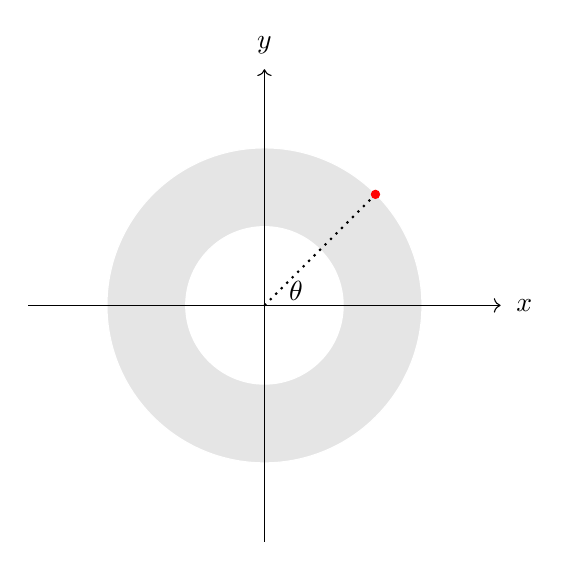
\begin{tikzpicture}

        % Define center points
        \filldraw[fill = black!10, draw = black!0] (0,0) circle(2);
        \filldraw[fill = white!100, draw = white!100] (0,0) circle(1);
        \draw[->] (-3,0) -- (3,0);
        \draw[->] (0,-3) -- (0,3);
        \draw[dotted, thick] (0,0) -- (1.41,1.41);
        \node[fill = red, circle, inner sep = 1.2] (pt) at (1.41,1.41) {};
        \node (theta) at (0.4,0.18) {$\theta$};
        \node (x) at (3.3,0) {$x$};
        \node (y) at (0,3.3) {$y$};
    \end{tikzpicture}
    \caption{The Torus viewed from above}
    \end{subfigure}
    \begin{subfigure}[b]{0.4\textwidth}
        \centering
        \begin{tikzpicture}

            % Define center points
            \draw[black] (0,0) circle(2);
            \draw[->] (-3,0) -- (3,0);
            \draw[->] (0,-3) -- (0,3);
            \draw[dotted, thick] (0,0) -- (1.41,1.41);
            \node[fill = red, circle, inner sep = 1.2] (pt) at (1.41,1.41) {};
            \node (theta) at (0.4,0.18) {$\phi$};
            \node (x) at (3.3,0) {$x$};
            \node (z) at (0,3.3) {$z$};
        \end{tikzpicture}
    \caption{One ring of the Torus viewed from the side}
    \end{subfigure}
      \caption{A description of a point on the Torus with two rotational coordinates.}
      \label{fig:Q5_Torus_Coords}
\end{figure}

Now for some fixed angle $\rho$ one can define the map $v_\rho:S^1 \times S^1 \rightarrow S^1 \times S^1$ 
which sends $(\theta,\phi)$ to $(\theta+\rho,\phi)$. This map clearly does not fix any points 
in $S^1 \times S^1$. Now consider the map $r_\rho \circ v_\rho:S^1 \times S^1 \rightarrow \mathbb{R}^3$ 
as the map which rotates all points on the Torus by some fixed angle and then moves all points 
outward so that they lie on their respective tangent planes (see \autoref{fig:Q5_Torus_Map}).

\begin{figure}[H]
    \centering
    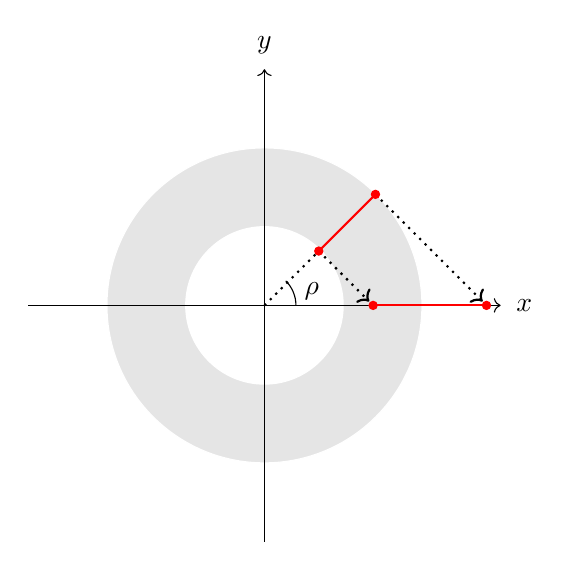
\begin{tikzpicture}

        % Define center points
        \filldraw[fill = black!10, draw = black!0] (0,0) circle(2);
        \filldraw[fill = white!100, draw = white!100] (0,0) circle(1);
        \draw[->] (-3,0) -- (3,0);
        \draw[->] (0,-3) -- (0,3);
        \draw[dotted, thick] (0,0) -- (0.7,0.7);

        \draw[->,dotted, thick] (0.69,0.69) -- (2*0.69-0.05,0.05);
        \draw[->,dotted, thick] (1.41,1.41) -- (2*1.41-0.05,0.05);

        \draw[thick, red] (0.7,0.7) -- (1.41,1.41);
        \node[fill = red, circle, inner sep = 1.2] (pt) at (1.41,1.41) {};
        \node[fill = red, circle, inner sep = 1.2] (pt) at (0.69,0.69) {};

        \draw[thick, red] (2*0.69,0) -- (2*1.41,0);
        \node[fill = red, circle, inner sep = 1.2] (pt) at (1.41+1.41,0) {};
        \node[fill = red, circle, inner sep = 1.2] (pt) at (0.69+0.69,0) {};

        \draw (0.4,0) arc(0:45:0.44);
        \node (theta) at (0.6,0.18) {$\rho$};
        \node (x) at (3.3,0) {$x$};
        \node (y) at (0,3.3) {$y$};
    \end{tikzpicture}
    \caption{The action of $r_\rho \circ v_\rho$ on a circular subset of the Torus (red) 
    viewed from above}
    \label{fig:Q5_Torus_Map}
\end{figure}

It is hopefully clear that $r_\rho$ is a continuous function, so $r_\rho \circ v_\rho$ is a 
continuous function that maps every point on the Torus to a point in its tangent plane but 
maps no points to themselves.






\end{document}
